\documentclass[11pt,a4paper]{article}
\usepackage[utf8]{inputenc}
\usepackage[T1]{fontenc}
\usepackage[romanian]{babel}
\usepackage[margin=2cm]{geometry}
\usepackage{array}
\usepackage{tabularx}
\usepackage{enumitem}
\usepackage{graphicx}
\usepackage{setspace}
\usepackage{xcolor}
\usepackage{hyperref}
\usepackage{amssymb}
\setlength{\parindent}{0pt}
\newcommand{\fillline}[1][6cm]{\underline{\hspace{#1}}}
\newcommand{\fillbox}[1][0.4cm]{\framebox[#1]{\rule{0pt}{#1}}}
\newcommand{\checkboxempty}{$\square$}

\begin{document}

\noindent
\begin{minipage}[t]{0.40\textwidth}
\vspace{0pt}
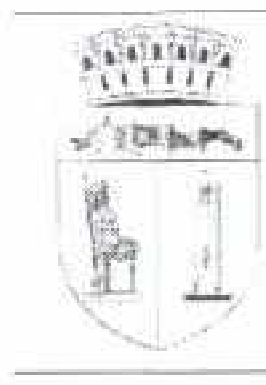
\includegraphics[height=1.5cm]{../assets/stema-cluj.png}%
\hspace{0.2cm}%
\raisebox{0.5cm}{\parbox[t]{3.5cm}{\textbf{PRIMĂRIA}\\\textbf{CLUJ-NAPOCA}}}
\end{minipage}%
\begin{minipage}[t]{0.30\textwidth}
\centering
\vspace{0.4cm}

\includegraphics[width=3.5cm,height=0.9cm]{../assets/barcode-311006.png}
\end{minipage}%
\begin{minipage}[t]{0.30\textwidth}
\raggedleft
\vspace{0.6cm}
Nr. \fillline[3cm] / \fillline[1cm]
\end{minipage}

\vspace{0.5cm}

\begin{flushright}
\underline{\textbf{ANEXA Nr. 5}}
\end{flushright}

\vspace{0.5cm}

\begin{flushright}
\begin{tabular}{l}
DATĂ ÎN FAŢA MEA, \\
\fillline[6cm] \\
la data de \fillline[5cm] \\
semnătura \fillline[5cm] \\
\end{tabular}
\end{flushright}

\vspace{1cm}

\begin{center}
\textbf{D E C L A R A Ţ I E}
\end{center}

\vspace{0.5cm}

Subsemnatul(a) \fillline[10cm] fiul(fiica) lui \fillline[6cm] şi al \fillline[6cm] născut(ă) la data de \fillline[4cm] în localitatea \fillline[5cm] judeţul \fillline[4cm] posesor al actului de identitate seria \fillline[1.5cm] numărul \fillline[3cm] proprietar al locuinţei din \fillline[5cm] str. \fillline[6cm] nr. \fillline[1.5cm] bl. \fillline[1.5cm] sc. \fillline[1.5cm] etj. \fillline[1.5cm] apt. \fillline[1.5cm] sector \fillline[1.5cm] având actul de spaţiu (denumirea) \fillline[5cm] nr. \fillline[2cm] din \fillline[2.5cm] emis de \fillline[3cm] \fillline[4cm] declar că primesc în spaţiul meu de locuit pe \fillline[6cm] fiul (fiica) lui \fillline[5cm] şi al \fillline[6cm] nascut(ă) la data de \fillline[4cm] în localitatea \fillline[5cm] judeţul \fillline[4cm] cu ultimul domiciliu în localitatea \fillline[4cm] str. \fillline[5cm] nr. \fillline[1.5cm] bl. \fillline[1.5cm] sc. \fillline[1.5cm] etj. \fillline[1.5cm] apt. \fillline[1.5cm] sector \fillline[2cm] în calitate de \fillline[4cm]

\vspace{0.3cm}

Dau prezenta declaraţie pentru a-i servi numitului(ei) \fillline[8cm] la schimbarea domiciliului în spaţiul de locuit de la adresa mai sus amintită.

\vspace{2cm}

Data \fillline[4cm] \hfill Semnătura \fillline[5cm]

\vfill

\hrule
\vspace{0.2cm}
\footnotesize
www.primariaclujnapoca.ro\\
telefon: 0264/596.030\\
Cluj-Napoca, str. Moţilor, nr. 3

\vspace{0.3cm}

Timp estimativ de completare: 10 minute

Datele personale care vă sunt solicitate prin prezenta cerere vor fi prelucrate numai în vederea procesării și soluționării solicitării dumneavoastră. Primăria municipiului Cluj-Napoca garantează securitatea procesării datelor și arhivarea acestora în conformitate cu prevederile legale în vigoare. Responsabilul Primăriei municipiului Cluj-Napoca cu protecția datelor poate fi contactat pe adresa de email dpo@primariaclujnapoca.ro.

În conformitate cu Regulamentul nr. 679/2016 aveți dreptul de a solicita Primăriei municipiului Cluj-Napoca, în ceea ce priveşte datele cu caracter personal referitoare la persoana vizată, accesul la acestea, rectificarea sau ştergerea acestora sau restricţionarea prelucrării sau a dreptului de a vă opune prelucrării, precum şi a dreptului la portabilitatea datelor.

\end{document}
